%                         File: osa-revtex4-1.tex                             %
%                        Date: April 15, 2013                                 %
%                                                                             %
%                              BETA VERSION!                                  %
%                   JOSA A, JOSA B, Applied Optics, Optics Letters            %
%                                                                             %
%            This file requires the substyle file osajnl4-1.rtx,              %
%                   running under REVTeX 4.1 and LaTeX 2e                     %
%                                                                             %
%                   USE THE FOLLOWING REVTeX 4-1 OPTIONS:                     %
% \documentclass[osajnl,twocolumn,showpacs,superscriptaddress,10pt]{revtex4-1}%
%                    %% Use 11pt for Applied Optics                           %
%                                                                             %
%               (c) 2013 The Optical Society of America                       %
%                                                                             %
%%%%%%%%%%%%%%%%%%%%%%%%%%%%%%%%%%%%%%%%%%%%%%%%%%%%%%%%%%%%%%%%%%%%%%%%%%%%%%%
% Uses bib file and needs bibtex stuff.  Once ready, insert .bbl file created
% by this into the hand-inserted bibliography to get final OE submission.
% Why is this necessary?? 

\documentclass[review]{elsarticle}

\usepackage{lineno,hyperref}
\modulolinenumbers[5]
\usepackage{color}
\usepackage{amsmath}
%%%%%%%%%%%%%%%%%%%%%
% REMOVE BEFORE SUBMISSION
\usepackage{amsmath,amssymb,graphicx}
\usepackage{dcolumn}%
\usepackage{array,multirow}
\usepackage{bm}%
%\usepackage{cite}
\usepackage{pstool}%
\usepackage{array}
\usepackage{xcolor}
\usepackage{subcaption,subfloat} % lets you have multiple pictures next to each other
%\usepackage{upgreek}
%\usepackage[numbers,sort&compress]{natbib}
\newcommand{\beginsupplement}{%
        \setcounter{table}{0}
        \renewcommand{\thetable}{A\arabic{table}}%
        \setcounter{figure}{0}
        \renewcommand{\thefigure}{A\arabic{figure}}%
     }
\journal{Solar Energy}
\bibliographystyle{elsarticle-num}

\begin{document}
\begin{frontmatter}
\title{Optical nanostructures design, fabrication, and applications for solar/thermal energy conversion } %Title of paper

\author{Mool C. Gupta,$^{1,*}$ Craig Ungaro,$^1$ 
Jonathan J. Foley IV,$^{2}$ and Stephen K. Gray$^{3,\dagger}$}

\address{$^1$Department of Electrical \& Computer Engineering, University of Virginia, Charlottesville, Virginia, 22901, USA \\
$^2$Department of Chemistry, William Paterson University, 300 Pompton Road, Wayne, NJ, 07470, USA \\
$^3$Center for Nanoscale Materials, Argonne National Laboratory, 9700 South Cass Avenue, Argonne, IL, 60439, USA \\
$^*$mgupta@virginia.edu \\
$^{\dagger}$gray@anl.gov}


\begin{abstract}
Optical nanostructures can control the optical absorption and emission properties of surfaces and are therefore being investigated for solar thermophotovoltaics, thermophotovoltaics, solar thermal, infrared sensing, infrared sources, incandescent light sources, and thermal imaging applications, among many others. This review article describes various modeling methods available for design of 
optical nanostructures to control light absorption and emission properties of surfaces, as well as various methods available for the fabrication of large area nanostructured surfaces. Throughout the review, we provide examples of state of the art energy generation devices using such 
optical nanostructures.  A discussion of outstanding obstacles for the achievement of high efficiency solar thermophotovoltaics systems is provided along with examples of systems showing exceptional promise. 
\end{abstract}

\begin{keyword}
Optical design and fabrication \sep Optical Devices \sep Optics at surfaces \sep Thin Films \sep Solar Energy \sep Subwavelength structures, nanostructures
\end{keyword}



%\begin{keyword}
%\ocis{(220.022) Optical design and fabrication; (230.023) Optical devices;  (240.024) Optics at surfaces; (240.031) Thin films; (350.605) Solar Energy; (310.662) Subwavelength structures, nanostructures.}
%\end{keyword}

\end{frontmatter}
%\ocis{350.6050}% REPLACE WITH CORRECT OCIS CODES FOR YOUR ARTICLE
%                          % NOTE: \ocis{} IS ALIASED TO \pacs{} BUT MUST
%                          % FORMAT THE TERMS CORRECTLY FOR EACH JOURNAL

%%%\maketitle %% required
\linenumbers

\providecommand{\noopsort}[1]{}\providecommand{\singleletter}[1]{#1}%
               

\section{Introduction}
Recently, there has been strong research activity in solar thermal (ST) \cite{g1,g2}, solar thermophotovoltaic (STPV) \cite{g3,g4,g5,nnn1}, and thermophotovoltaic (TPV) \cite{g6,g7} energy conversion.  To provide a state of the art status in 
these fields, we have prepared this review article.  There is strong potential for growth in these areas, especially 
through the use of novel nanostructured surfaces to control light absorption and emission from surfaces and to 
achieve high efficiency. This spectral light control can be achieved by nanostructuring of surfaces, 
which can strongly modify their optical properties \cite{g8,g9,RF_OptExp_2009}. Recently, significant progress has been made in the modeling and fabrication of nanostructures to control optical absorption and emission properties of surfaces. 
Nanostructured surfaces, for example, can be designed to be significantly
more absorbing than their flat counterparts.
Similarly, surfaces can be designed to emit infrared radiation in a very narrow spectral range, providing spectrally selective 
surfaces~\cite{G_PS_1985, C_RPP_2014}.  Figure \ref{gfig_bbs} shows the change in 
emission spectra from a blackbody emitter to a selective emitter using optical nanostructures.
Some typical nanostructures are depicted schematically in Fig. \ref{gfig_surfs}.

STPV, ST, and TPV systems all share common surfaces but operate under different conditions.  ST and STPV systems offer an alternative to PV power generation in alternative energy systems.  Since both are heat engines, they do not adhere to the Shockley-Queisser limit and can theoretically exhibit extremely high efficiencies.  Additionally, since both ST and STPV systems rely on elements heated to high temperatures via concentrated solar energy, they are easy to modify for thermal storage of energy~\cite{SteadyStateAnalysis,Night_time_Performance}.  This would allow them to operate into the night.  An advantage of ST systems over STPV systems is that ST systems do not require the use of PV cells.  The PV cells in STPV systems are expensive and can limit overall system size.  Conversely, an advantage of STPV systems over ST systems is that STPV systems have no thermal fluid or moving parts.  This leads to them being more stable and compact solutions.  Overall, ST tends to lend itself to large, immobile power installations while STPV is better suited for small applications.  TPV systems operate on the same principle as STPV systems, but rely on an external heat source instead of solar energy~\cite{Prototype_TPV}.  This allows them to be used in energy reclamation systems.

\begin{figure}[ht!]
	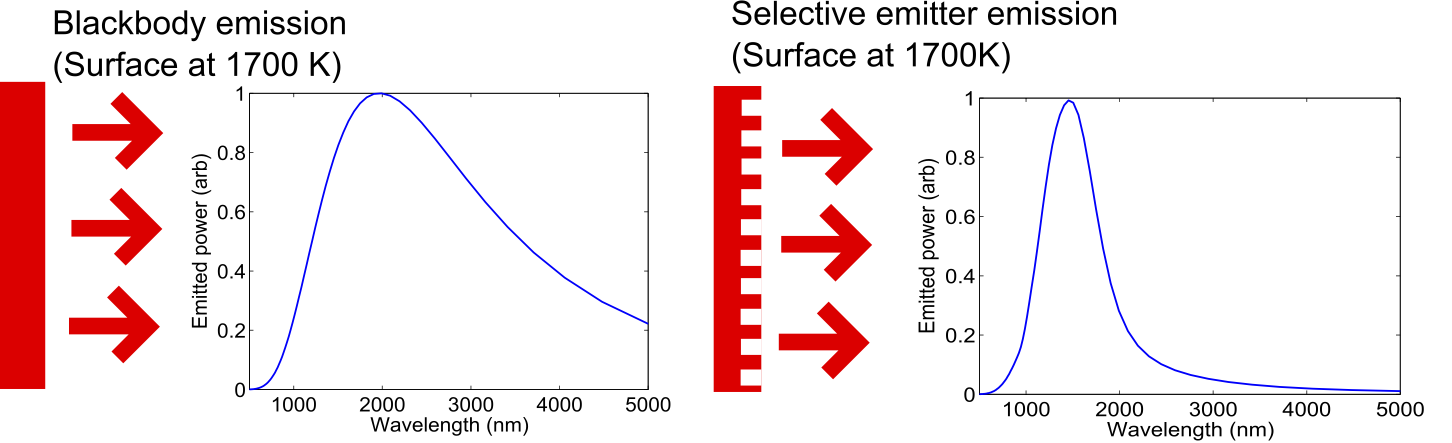
\includegraphics[width=1\textwidth]{gfig_bbs}
	\caption{\label{gfig_bbs} Spectral emission of a blackbody vs. a selective emitter.  Note that the scales on each graph are in different arbitrary units; the graph is intended to show the relative narrowness of the spectrum using the selective emitter.}
\end{figure}

\begin{figure}[ht!]
	
\includegraphics[width=1\textwidth]{gfig_surfs}
	\caption{\label{gfig_surfs} Types of nanostructured absorbing and 
emitting surfaces: a) random nanotexture b) periodic nanotexture and c) dielectric/metal stack.} 
\end{figure}

Such control of light absorption and emission properties allows the design of high efficiency solar and thermal energy conversion devices. It also has applications in the development of 
high efficiency infrared sources, sensors, and incandescent light sources. 
Various approaches have been demonstrated for controlling light absorption and emission 
from surfaces such as the use of photonic crystals \cite{g11,NYL_SEMSC_2014,g13,g14}, 
optical metamaterials \cite{g15,g16,g17}, nanoparticles \cite{g18,g19,g20,g21}, 
multilayer thin films \cite{g22,RF_OptExp_2009} and micro/nano textured 
structures \cite{g25,g26,g27,g28}.  This review article describes various modeling methods 
available for design of optical nanostructures to control light absorption and emission properties of surfaces, the various methods available for the fabrication of large area nanostructured surfaces, and provides some examples of high-efficiency, state of the art, energy generation devices using such optical nanostructures.  A path forward to more efficient solar and thermal energy generation devices using practical design methods and fabrication techniques is examined.

The limiting efficiency for ST and STPV systems with ideal absorbing and emitting surfaces comes from the Carnot efficiency ($\eta$) 
given by $\eta = 1 - \frac{T_c}{T_h}$, where $T_c$ and $T_h$ are the hot and cold temperatures, respectively. The absorbing 
surface efficiency is lowered due to radiative loss, 
given by $ A \epsilon \sigma T^4$, where $A$ is the area, $\epsilon$ is emissivity, $\sigma$ is the Stefan-Boltzmann constant, and $T$ is temperature.  
While the Carnot efficiency of the system will increase with temperature, the absorbing surface efficiency will decrease due to 
increased emission from the absorbing surface at high operating temperatures~\cite{L_AIP_2007}.  The maximum operating efficiency 
of 85.4\% is therefore reached at an operating temperature of 2600 K in the ideal case for both systems.  Increasing 
the temperature beyond this will result in a decrease in system efficiency.  This analysis assumes that incoming 
radiation is concentrated to the maximum achievable solar concentration of 46000x.  At this concentration, the 
ideal surface is simply a blackbody absorber.
 
As the solar concentration is decreased, the ideal surface will be a blackbody absorber for wavelengths below 
some $\lambda_{cutoff}$, and an ideal reflector (generating lower emission) for wavelengths above the cutoff.  The 
location of $\lambda_{cutoff}$
depends on the temperature of the system, the power density of the emission from the emitter, and the solar concentration 
levels achieved in the system.  Typical $\lambda_{cutoff}$ values will be close to 2 $\mu m$ due to the importance of absorbing a 
large portion of the solar spectrum~\cite{RF_OptExp_2009}.
 
In the case of STPV systems, the emitting 
surface will also play a role in device efficiency.  The ideal
surface will be a monochromatic emitter that emits radiation with energy equal to the 
bandgap energy of the PV cell used in the system~\cite{TheoreticalEfficiency,L_AIP_2007}.  Unfortunately, monochromatic 
emitters have a power density of 0, resulting in the requirement of an infinitely large 
emitting surface for practical power generation.  Therefore, in practical STPV systems, an 
emitting surface with a small bandwidth will be desirable~\cite{RF_OptExp_2009}.  
Figure~\ref{Ideal} 
shows the evolution of maximum system efficiency vs. temperature for an ideal system.
\begin{figure}[ht!]
\begin{center}
        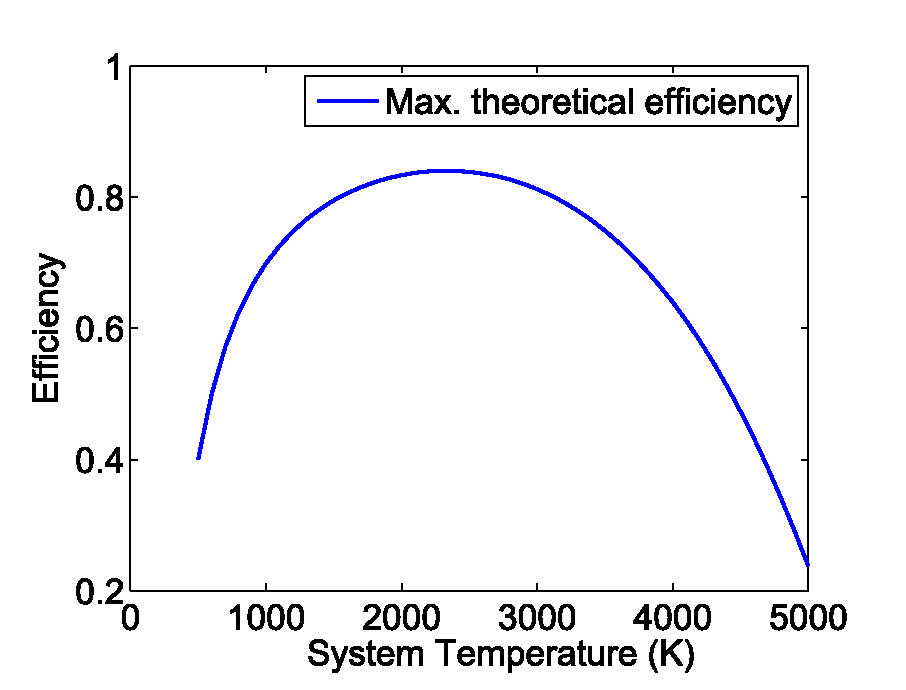
\includegraphics[width=0.5\textwidth]{ideal_STPV_eff}
        \caption{\label{Ideal} Maximum theoretical efficiency for various system temperatures.  Note the fast increase
around typical operation temperatures for ST and STPV systems.}
\end{center}
\end{figure}

The temperature of 1000$^\circ$C was an upper limit chosen for practical ST systems based off existing 
technologies~\cite{RKR_RenEnRev_2013, g2}.  This temperature was chosen for the purpose of comparing different nanostructured 
surfaces suitable for incorporation into ST systems.  The performance of ST systems will generally 
increase up to a specific temperature~\cite{MS_EnConvMan_2012}.  The value of this temperature is dependent on the 
quality of surfaces used and the solar concentration value achieved.  For tower-based (high-concentration) 
ST systems, this temperature is usually significantly above current operating temperatures, resulting in a 
desire for increased thermal stability. Most materials degrade at high temperatures for extended period of 
operation, so a reasonable number of 1000$^{\circ}$ was assumed. This number is consistent with temperature used in 
many solar thermal applications as well as for thermophotovoltaics.

Figure \ref{gfig_surfs} shows different kinds of nanostructures used to create spectrally selective surfaces in energy generation systems.  Random and periodic nanostructures may have different shapes depending on the fabrication method used.  Triangular, sawtooth, square, spherical, and cylindrical structures all see use in these systems \cite{global_opt,paper2_ref6,RF_OptExp_2009}.  Additionally, spherical or obloid nanostructures may be embedded in a dielectric matrix to selectively scatter specific wavelengths of light.  Lastly, as shown in Figure 2c, planar dielectric or dielectric and metal stacks may be used.

Melting point depression and thermal mismatching between layers makes temperature stability a major concern for spectrally selective surfaces.  This issue is solved primarily through material selection and the use of protective coatings on nanostructured materials \cite{paper1_ref5}.  Smaller nanostructures and thinner layers can increase this effect, resulting in a limited design space for some nanomaterials.

The type of nanostructure used in a system can have a large impact on its ease of fabrication, spectral selectivity, and temperature stability.  The use of random elements in nanostructures eases fabrication tolerance requirements and can improve selectivity, but can be difficult to design for or simulate properly \cite{me1}.  The presence of some smaller--period nanostructures can lead to lower thermal stability in random nanostructures as well. 

Square and cylindrical type gratings result in a rapid change in index of refraction (as compared to tapered structures) that can result in low visible or near infrared (IR) emittance and narrow absorption peaks \cite{paper1_ref6,paper2_ref13}.  This can be a boon to the design of narrow-band emitter structures, or a hindrance to the design of solar absorbing surfaces.  Combinations of multiple periods of gratings can be used to broaden the emittance peaks in these structures; however, they still lack high emission in the near IR and visible regions \cite{paper2_ref14}.  Using conical, sawtooth, or triangular type nanostructures can increase short-wavelength emission due to the more gradual change in index throughout the structure \cite{Grann_JOSA,me2}.
Planar surfaces using thin layers of multiple different dielectrics suffer from relatively broad absorption peaks.  The inclusion of a metallic layer or the addition of many dielectric layers can result in a much more narrow emission peak \cite{RF_OptExp_2009}.  


There are many examples in the literature of nanostructures being applied to make high efficiency systems.  Wang {\it et al.} \cite{g15} have demonstrated a highly efficient selective metamaterial absorber for high-temperature solar thermal energy harvesting. Using nanostructured titanium gratings on a MgF$_2$ spacer deposited on W thin films was demonstrated with UV-near IR absorption of 0.9 and mid-IR emittance of 0.2.  
A structure with solar to heat conversion efficiency of 80\% at 400$^\circ$C was 
modeled and fabricated to achieve high solar light absorption efficiency over broad spectral wavelength range and emission surfaces emitting in a narrow band of wavelengths. 

Spectrally selective surfaces have also been achieved by depositing nanoparticles on a 
surface and 
modifying surface morphology.  Shah {\it et al.} \cite{g21} investigated spectrally 
selective surfaces for concentrated solar power 
receivers by laser sintering of tungsten micro and nanoparticles on a stainless steel 
substrate, resulting 
in a solar absorptance of 83\% and thermal emittance of 11.6\% at 
room temperature.  Multi-layer thin films of metal-dielectric coatings have also been shown to provide high broad wavelength solar absorption and low thermal emittance \cite{g22}.

The use of theory and modeling has been critical to the design of these types of record-breaking
structures, and will no doubt be critical moving forward as the community continues to push
the limits of conversion efficiency, durability, affordability, etc.
In the following section, we will try to illustrate how theoretical electrodynamics techniques
can be brought to bear to design these types of structures, as well as what challenges exist.

\section{Design methodologies}

\subsection{Overview of the theoretical foundations of the optical properties of nanostructures}

Understanding how a nanostructured surface or particle absorbs, scatters, and/or reflects incident light provides
critical information enabling the design of systems for efficient solar
energy conversion.  Calculating these quantities depends upon the ability to solve Maxwell's
equations when light is incident upon nanostructures~\cite{G_JPCC_2013}.   A wide variety of theoretical 
methodologies exist for solving Maxwell's equations either in the time-domain (see for example 
\cite{Taflove_FDTD,Meep}), 
or in the frequency domain (see for example~\cite{Bohren,Yeh,DF_JOptSocA_1994,fem,RCWA1,RCWA2}). 
Time-dependent approaches of solving Maxwell's equations 
typically start from the first-order time-dependent electric
and magnetic field equations,  whereas frequency domain methods usually take the second-order frequency-dependent wave equation, 
supplemented by appropriate boundary conditions, as their starting point.

In a few cases, Maxwell's equations  can be solved analytically; indeed, under some often
reasonable approximations, the analytical solutions can even be written simply, which
greatly aids intuition about the behavior of a nanostructure.  Two important analytical examples we will
consider include the interaction of light with spherical nanostructures, solvable by Mie
theory, and the interaction of light with planar nanostructures, solvable by the Transfer
Matrix method.   For more general structures, numerical techniques must be employed, and
several approaches have been put to considerable use.  Here we will
discuss the finite-difference time-domain (FDTD) method and the discrete dipole
approximation (DDA); the former solves Maxwell's equations in the time-domain, while the 
latter
solves them in the frequency-domain.  The finite element method, or FEM, is a  
frequency-domain approach capable of describing a greater variety of problems~\cite{fem}.
The vectorial
nature of Maxwell's equations make
implementations of FEM significantly more sophisticated than DDA.  Rigorous coupled-wave analysis (RCWA) represents
another frequency-domain method for solving Maxwell's equations that is particularly relevant for periodic structures~\cite{RCWA1,RCWA2} and, because of its efficiency, has been used successfully to design
absorber and emitter structures for TPV/STPV applications, see for example~\cite{A13, RCWA3}.  We will also give several
examples of applications of nanostructures for
solar energy conversion, focusing on which of the above methodologies are most
appropriate, and how they would be utilized for designing these nanostructures.

\subsection{Mie theory for spherical nanostructures}
Mie theory provides an analytical solution for Maxwell's equations when light is incident
upon a spherical particle. Analytical solutions are available for not only
homogeneous spheres but spheres composed of a core sphere with one or more outer shells, and
arbitrary complex dielectric constants may be used to define the spherical systems.   
Quantities like the absorption, scattering, and extinction cross section of the particle
can be easily computed with Mie theory. 
An excellent
discussion of Mie theory, as well as practical source code, can be found in~\cite{Bohren}.

While only rigorous for 
isolated spherical particles in homogeneous media, judicious use of Mie theory can be an invaluable tool for modeling more complicated structures.  For instance, Mie theory can 
be adapted for very small particles that can be modeled as ellipsoids, which includes nanodisks, 
nanorods, etc.~\cite{Bohren}  Similarly, Mie theory 
can be combined with effective medium theories, e.g. Maxwell-Garnett theory, to model 
regular or random arrays of particles on a substrate, provided that the coupling 
between the neighboring particles is negligible~\cite{Bohren}.  
Extensions to effective medium theories have also
been developed that account for the impact on near-neighbor coupling on the 
polarizability of a spherical structure, 
including renormalized polarizability approaches of Moch\'{a}n and co-workers\cite{BCM_PRB_1988,BMM_PRB_1991}, and dressed
polarizability approaches of Yoo {\it et al.}\cite{YP_OptExpress_2012}.  These approaches offer similar simplicity of
using Mie theory in conjunction with an effective medium theory, but offer a more rigorous treatment of the coupled
optical response of the spherical particle to its neighbors. 

\subsection{Design of nanostructures for enhancing solar energy conversion using Mie theory}
The relative simplicity of the theoretical framework describing scattering and absorption of spherical 
nanostructures affords the ability to design
systems utilizing spherical nanoparticles for a variety of solar conversion applications.  The scattering properties of
spherical nanoparticles can be leveraged to concentrate and trap incident light into thin-film photovoltaic (PV) materials to increase their
conversion efficiency.  This strategy is particularly effective if the light scattering can occur only in the forward direction, increasing
the flux of optical energy into an active PV material, for example~\cite{AP_NatMat_2010}.
Mie theory
leads to the prediction of this particularly extreme form of anisotropy where the particles scatter light only in the
forward direction when the coefficients for the electric and magnetic dipolar terms are identical, which is often called the first Kerker condition~\cite{GGG_NatComm_2012}.
Physically, this can be understood as an interference between electric
and magnetic dipolar resonances.   Because this is a resonant effect, a given particle geometry will support such scattering behavior
only at certain frequencies.  Nevertheless, Mie theory computes these coefficients directly, and it is straightforward to develop a
design protocol for spherical particles embedded in a medium with known optical properties (e.g. corresponding to the PV material, or a
compatible substrate) that support these resonances at a desired frequency.  The exceptionally large extinction cross sections
of metal nanoparticles, due to their ability to support surface plasmons, can also be exploited to efficiently trap light across
the solar spectrum.  For example, the optical response of spherical dielectric-core metal-shell nanoparticles is highly tunable, and can be
computed exactly with a generalization of Mie theory.  Halas and co-workers have employed Mie theory to
design optimal distributions of core-shell nanoparticles to enhance absorption over the AM 1.5 solar 
spectrum~\cite{CH_APL_2006}, where AM 1.5 indicates the standard for the solar 
spectrum after attenuation by Earth's atmosphere.
Using a distribution of simple silica core/gold shell particles with modest coverage allowed absorption of 84\% of incident solar power
across the AM 1.5 spectrum~\cite{CH_APL_2006}.  Figure~\ref{Halas} shows the extinction efficiency computed
by Mie theory for various core-shell particle structures.  
Similarly, resonant or near-resonant scattering effects of spherical or cylindrical 
nanostructures, including nanowires, have been modeled within the framework of Mie theory to create exceptionally strong broad-band absorbing structures~\cite{FKA_OptExp_2014}
and broad-band anti-reflection coatings~\cite{SVP_NatComm_2012}, both of which are 
widely applicable to solar conversion technologies.  Again, we emphasize that Mie theory is rigorous only in the limit of isolated particles, 
and cannot easily account for particle/interface effects.
For such effects, more general numerical modeling approaches such as FDTD or DDA are required, and we discuss these approaches in Sections 2.6-2.8.

\begin{figure}[ht!]
\begin{center}
        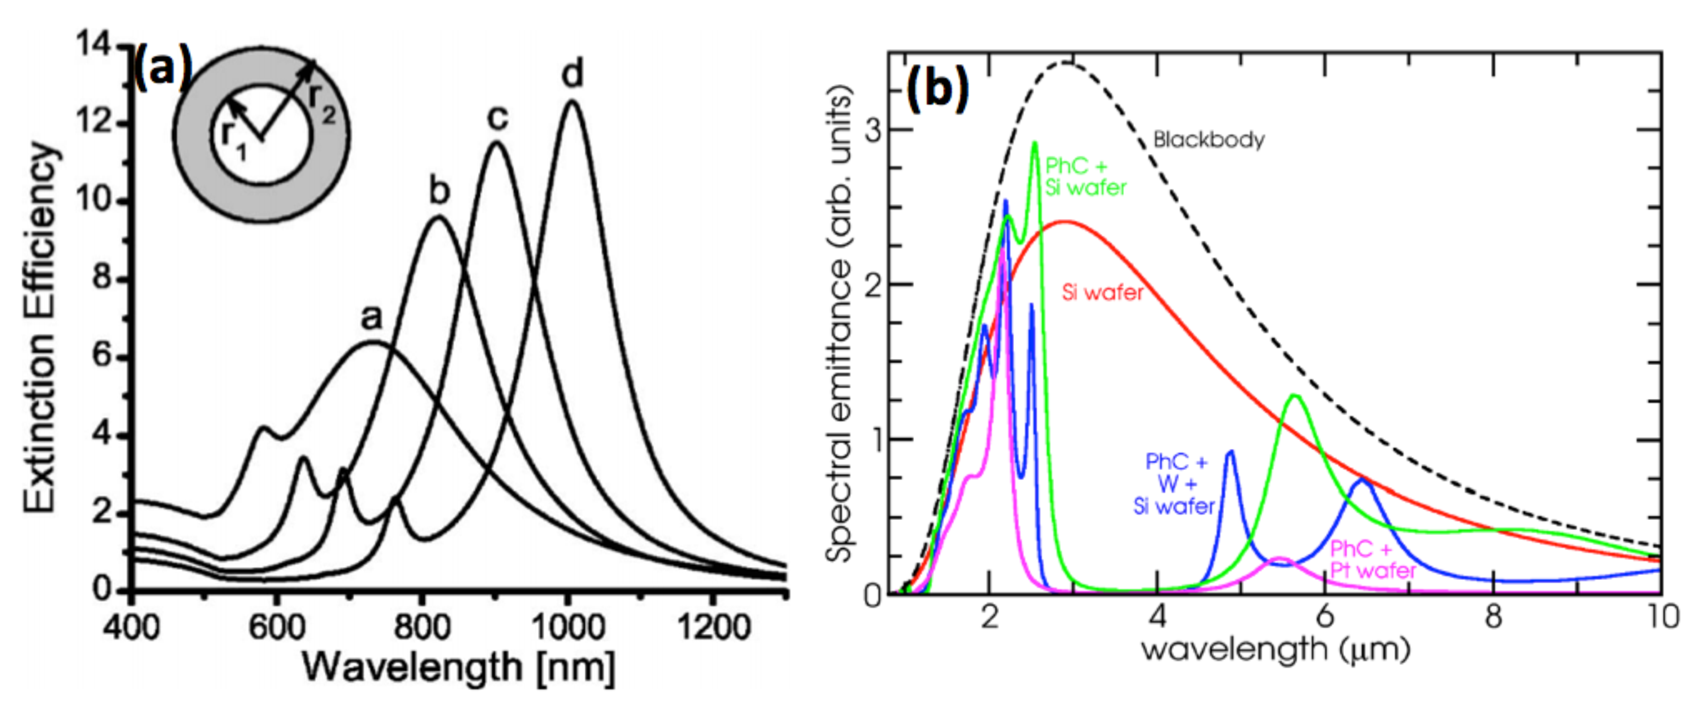
\includegraphics[width=\textwidth]{Halas_Celanovic}
        \caption{\label{Halas}  Illustration of radiation control using engineered spherical core-shell
nanoparticles {\bf (a)} and multi-layer planar film structures {\bf (b)}.
The absorption, scattering, and extinction cross sections of the core-shell particles can be tuned
across the solar spectrum by changing the ratio of the shell thickness ($r_2$) to the core radius ($r_1$), 
and these
quantities can be computed using Mie theory (see Section {\it 2.2}) for isolated particles, or the 
DDA method (see Section {\it 2.8}) for assemblies of particles.
In {\bf (a)}, the radius of a silica core is fixed at 60 nm, and the thickness of a gold shell is
taken to be 80 nm for curve {\bf a},
70 nm for curve {\bf b}, 67 nm for curve {\bf c}, and 65 nm for curve {\bf d}.
The emittance of several multi-layer structures plotted in {\bf (b)} can be simply computed
using the Transfer Matrix Method (see Section {\it 2.4}); however, 
more sophisticated global device
efficiency considerations were used to identify a photonic crystal on a platinum substrate 
(violet curve in {\bf (b)} as the optimal emitter structure for
an integrated STPV system~\cite{g4}.
Figures reproduced from~\cite{CH_APL_2006} and~\cite{g4} with permission.}
\end{center}
\end{figure}

\begin{figure}[ht!]
	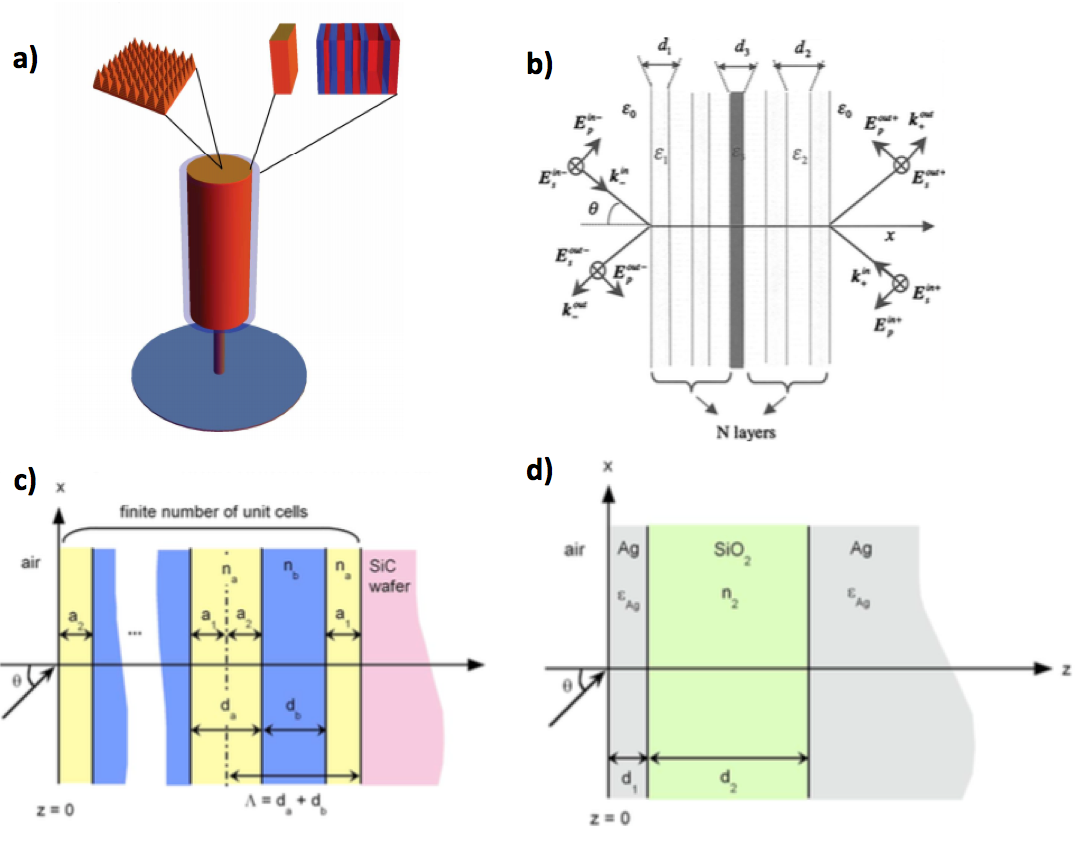
\includegraphics[width=\textwidth]{Planar}
	\caption{\label{Fan}  Illustration of various planar structures amenable to design and modeling
by transfer matrix methods that serve as selective emitter structures.  
A 1D photonic crystal integrated into a STPV absorber/emitter structure is  
is illustrated in {\bf (a)}. Further details, including absorptivity spectra from this class of structures, can be found
in Fig. 6 and in~\cite{paper1_ref4}.  A Bragg reflector with a single absorbing defect layer,
which supports spectrally selective emission modes, is illustrated in {\bf (b)}. Further details, including emissivity spectra from this class of
structures, can be found in~\cite{BN_JApplPhys_2005}.
A structure that achieves angular and spectral selectivity by coupling evanescent photonic crystal modes
to surface phonon polariton modes in a polar layer is illustrated in {\bf (c)}.  
A structure that achieves angular and spectral selectivity by coupling incident light into Fabry-P\'{e}rot
resonances is illustrated in {\bf (d)}.  Further details, including emissivity spectra from these classes of structures, can 
be found in~\cite{LZ_JApplPhys_2006}.  Figures reproduced from 
~\cite{paper1_ref4, BN_JApplPhys_2005, LZ_JApplPhys_2006} with permission.}

\end{figure}

\subsection{Transfer Matrix Methods for planar structures}
For multi-layer planar structures, the fields can be written piece-wise as plane waves, and closed-form expressions for the wavevectors
and amplitudes of the fields in each layer can be determined from considerations of Maxwell's equations and appropriate boundary
conditions.  The boundary conditions can be expressed conveniently as matrix equations, and the amplitudes can be computed by
straightforward matrix multiplication, which forms the basis of what is called the Transfer Matrix Method~\cite{Yeh}.  The general
Transfer Matrix equations for an $L$-layer system can be written as
\begin{equation}\label{Fresnel}
  \begin{pmatrix} E_1^+  \\ E_1^-  \end{pmatrix}
  \mbox{=}
  \begin{pmatrix}
  M_{1,1} & M_{1,2} \\
  M_{2,1} & M_{2,2}  \end{pmatrix}
  \begin{pmatrix} E_L^+ \\ E_L^-  \end{pmatrix},
\end{equation}
where the elements $M_{i,j}$ depend on the material properties (the refractive index, $n$) and geometry of each layer, as well as the
frequency and polarization of incident light.  The precise form of these elements can be found in the excellent treatment by Yeh~\cite{Yeh}, and this method 
has been successfully applied for designing multi-layer absorbing structures that find wide use in TPV/STPV applications~\cite{BN_JApplPhys_2005,LZ_JApplPhys_2006,FUS_OptExp_2015}.  We interpret $E_1^+$ and $E_1^-$
as incoming and outgoing wave amplitudes on the incident side, respectively; similarly, $E_L^-$ and $E_L^+$ are incoming and outgoing wave amplitudes, respectively,
on the terminal side of the structure.  With the access to the field amplitudes and wavevectors, a number of useful quantities may be computed.
For example, the Fresnel reflection and transmission amplitudes may be computed as $r =  E_1^-/E_1^+  =  M_{2,1}/M_{1,1}$  and
$t = E_L^+/E_1^+ =  1/M_{1,1}$, respectively.  The reflection can then be calculated as $R=|r|^2$, the transmission as
$T= |t|^2 \: n_L \: {\rm cos}({\rm Re}(\theta_L)))/(n_1 \: {\rm cos}(\theta_1))$, where $n_i$  and $\theta_i$ denote the refractive index of the material of layer $i$
and the incident/refraction angle in layer $i$, respectively.  For computing the Fresnel equations, 
the field amplitude $E_L^-$ is set to zero and the amplitude $E_1^+$ is set to 1 by convention.   
The absorption can simply be computed as $A= 1-T-R$.  An additional requiste assumption is that the semi-infinite bounding 
media (layer 1 and layer L) have real refractive indices.  When this is the case, $\theta_L$ will be a real angle to satisfy conditions
required by Snell's law for absorbing media~\cite{FMS_ACSPhoton_2014,CWH_JQSRT_2005} until the transmitted wave becomes evanescent, as is the case for total internal reflection
(when ${\rm Re}(\theta_L)=90^{\circ}$).  In this case, the transmission is necessarily zero, so the interpretation of the transmission ($T$), which must be a real number between 0 and 1, is preserved in the Transfer Matrix Method for absorbing intermediate materials bounded by semi-infinite dielectric layers.   That is, the Transfer Matrix Method allows all 
intermediate layers with finite thickness to have complex refractive indices and the fields to have complex angles of reflection/transmission 
in the intermediate layers.  Thus, the Transfer Matrix Method has been successfully applied for designing multi-layer absorbing structures that find wide use in TPV/STPV applications~\cite{BN_JApplPhys_2005,LZ_JApplPhys_2006,FUS_OptExp_2015}.
The computational effort of the Transfer Matrix Method is minimal as it primarily involves the computation of the matrix elements $M_{i,j}$, which can 
be accomplished in a number of arithmetic operations that scales linearly with the number of layers in the structure.
The Transfer Matrix Equations can also be used to compute the dispersion for resonant modes in multi-layer structures.  Two
resonant modes of particular interest for multi-layer structures with one or more absorbing layers include surface plasmon polariton 
(SPP) modes~\cite{WH_PSSb_1987,Maier,Novotny,AP_NatMat_2010,FHR_SciRep_2015}, 
and perfectly absorbing (PA) modes~\cite{DD_APL_2009,KSL_APL_2012,
KBG_NatMat_2013,FHR_SciRep_2015}.  SPP modes occur 
when $R \rightarrow \infty$ and   $T=0$, while the 
latter occurs
when $R \rightarrow 0$ and   $T=0$~\cite{FHR_SciRep_2015}.  SPPs involve collective electronic oscillations coupled to a propagating electromagnetic wave,
and they allow light to be guided along the 2-dimensional interface between a metal and a dielectric layer.  Because SPP wavevectors lie beyond the light-line (i.e. they have wavevector magnitudes larger than that of light propagating in the dielectric layer), excitation of SPPs can occur only under certain conditions.  A classic technique for exciting SPPs, known as the Kretschmann-Raether configuration~\cite{Raether},  involves an asymmetric dielectric/metal/dielectric structure with the refractive index of the dielectric substrate being larger than the refractive index of the dielectric superstrate.  While normally incident light cannot couple into SPPs on specular surfaces, it can couple into SPP modes at the metal/superstrate interface if it is incident from substrate side at an appropriate angle.  Using the Transfer Matrix Method to find the complex wavevector components that lead to the SPP condition ($R \rightarrow \infty$ and $T=0$) in such an asymmetric structure is equivalent to finding the angle that allows coupling of light into the SPP via Kretschmann-Raether excitation.~\cite{Raether, FHR_SciRep_2015}  Scattering at the surfaces, for example because of surface roughness or patterning with nanoparticles, can also produce large wavevector components that will allow light to couple into SPPs even at normal incidence.  Perfectly absorbing
modes can allow perfect absorption of incident light by thin absorbing layers.  Unlike SPPs, PA modes are 
non-propagating and do not necessarily lie to the right of the light line; in these cases, light can couple into perfectly absorbing modes in symmetric structures.~\cite{FHR_SciRep_2015}

\subsection{Design of selective emitters for thermophotovoltaic applications using Transfer Matrix Methods}
The resonant properties of multi-layer planar structures can be exploited for designing highly-selective emitter structures for use in
thermophotovoltaic (TPV) and STPV devices.  In TPV devices, thermal energy is transferred to a 
spectrally-selective emitter
structure.  The radiation wavelength of the emitter should be well matched to a PV cell bandgap so that its thermal emission can be efficiently converted
to electrical current.  TPV systems can harvest thermal energy as waste heat from engines or other sources.  An STPV system is simply 
a TPV system that harvests thermal energy from solar radiation, and involves a good solar absorber as one of its components.
The design of both absorbers and emitter structures has been the focus of considerable theory and modeling effort.
Figure~\ref{Fan} illustrates several optimized planar emitters that were designed using Transfer Matrix Methods~\cite{BN_JApplPhys_2005, LZ_JApplPhys_2006, RF_OptExp_2009}.

Despite their simplicity, multi-layer planar structures can support a rich number of interesting and controllable optical phenomena
which can be exploited for TPV and STPV applications.  One-dimensional photonic crystals (1DPCs) can be used in conjunction with absorbing
materials to enhance the spectral and/or angular selectivity of absorption and emission~\cite{paper1_ref4} in an integrated absorber/emitter STPV
structure.  The evanescent modes supported by 1DPCs
can also enable coupling into resonant surface waves in near and mid-IR frequencies, including surface plasmon polariton and surface
phonon polariton modes, respectively~\cite{LZ_JApplPhys_2006}, which gives hybrid 
structures consisting of hybrid 1DPCs and either a metal (strong near IR
absorber) or a polar material (strong mid IR absorber) 
exceptional angular and spectral selectivity.  Similarly, Ben-Abdallah and Ni have shown that coupling
between localized defect states and surface waves can give rise to strong spectrally coherent emission when a single absorbing defect layer is
introduced into a Bragg stack~\cite{BN_JApplPhys_2005}. The RCWA method has also been applied with success to both 1D and 2D periodic structures for selective absorber and emitter structures~\cite{A13, RCWA3}.  More details about the theory and implementation about this method can be found in~\cite{RCWA1, RCWA2}. 

Given the diversity of possible planar structures, a vast parameter space exists for their design, and optimization methodologies must
be chosen judiciously.  Drevillon and Ben-Abdallah~\cite{DB_JApplPhys_2007}, as well as Nafzaoui, Drevillon, and Joulain~\cite{NDJ_JApplPhys_2012},
have developed robust optimization 
methodologies that steer multilayer structures to an optimal emissivity profile. The optimum of the emissivity
profile can be defined in a variety of ways with respect to variables including the PV cell and operating conditions.
One such approach for defining such a profile involves using the spectral efficiency of the emitter as a figure-of-merit,
where the spectral efficiency depends on the emissivity of the structure, the band-gap of the PV cell, and the target 
temperature of operation (see section {\it 4.2}).  
The emissivity can be computed from the reflectance
and transmission using the Transfer Matrix Method, enabling efficient computation of the figure-of-merit.  The design problem can then be
formulated as a maximization of the figure-of-merit in terms of the geometry and material properties of the emitter structure.
This approach has been employed to design 1D photonic crystals involving tungsten and dielectric layers with spectral efficiencies of 
about 53\% ~\cite{SKY_JPE_2015} (see Table 2).  Similarly, the Transfer 
Matrix Method can be used to design broad-band absorbers, 
and has led to the prediction of 
absorption efficiencies of 74\% in 1D photonic crystals made of tungsten 
and dielectric layers~\cite{SKY_JPE_2015} (see Table 1).

A different Transfer Matrix Method-based approach for the design of STPV components, recently introduced by us, 
leverages the observation that structures that support perfectly absorbing modes with 
certain characteristics can perform as exceptional selective emitters.  These characteristics, described in detail in
~\cite{FUS_OptExp_2015}, can be
encoded directly into a search routine that allows for the identification of structure geometries that support these modes.  The
optimization over the figure-of-merit is therefore replaced with a search for a zero in T and R, which is equivalent to finding
a zero in the transfer matrix element $M_{2,1}$ under the condition that the transmission is also zero, which can be easily satisfied.
This approach has predicted structures with spectral efficiencies of 68\% at operating temperatures of 1750 K when coupled
with common PV materials~\cite{FUS_OptExp_2015}. The TMM has also been applied by Karalis and Joannopolous to the design of planar emitter/PV cell
systems separated by subwavelength gaps that exploit near-field radiative heat transfer effects, which can exceed the far-field
limit bounded by the Planck blackbody law~\cite{KJ_SciRep_2016}.  In their approach, the dispersions of the planar emitter and PV cell are designed
such that radiative coupling between the two is only allowed at a frequency just above the PV bandgap~\cite{KJ_SciRep_2016}.

\subsection{Finite-Difference Time-Domain method}

For the optical behavior of more general structures, numerical approaches must be employed to solve Maxwell's equations.  Perhaps the
most conceptually simple approach is known as the finite-difference time-domain (FDTD) method.  Here the time evolution of the fields
is computed using Maxwell's equations (the curl equations) where the spatial and temporal variables are discretized on a rectangular
grid, and centered finite-differences are used for the derivatives in terms of these variables~\cite{Taflove_FDTD}.
The electric and magnetic fields are spatially
staggered on the computational grid, which enforces Gauss' law.  Quantities such as absorption, scattering, reflection, and transmission
can be defined in terms of fluxes of electromagnetic fields.  Electric field distributions and other quantities may be obtained in the
frequency domain by the appropriate Fourier transform of the time-domain fields.  The permittivity of metals and semiconductors can
have strong frequency dependence across the UV/Vis/IR spectrum, and this frequency dependence requires some consideration for time-domain
simulations like FDTD.  
Material dispersion leads to time-dependence of the material susceptibility and 
causes the polarization
density to depend on field values at all previous times.  
This is commonly handled by fitting the permittivity to an analytical
function of frequency, commonly a sum of Drude and Lorentz oscillator functions, so that the convolution can be easily computed.  A
practical drawback is that it can be difficult to obtain a good fit for these functions across a broad spectrum for highly-dispersive materials.

The computational effort of FDTD scales with the 4$^{th}$ power of the computational domain for 
simulations with 3 spatial and 1 temporal dimension.
The spatial grids are generally discretized with grid spacing $d$, where $d$ is a value less
than the sub-wavelength electromagnetic field variations of interest in the complex
optical response media being studied. (In such media, suitable values of $d$ 
such that the results are converged must
be determined empirically.)
The time-step is usually defined relative to the spatial grid size by the Courant 
factor~\cite{Taflove_FDTD}.   This tends to make simulations of structures with several disparate length-scales challenging, as a small
grid size is required for the smallest feature, while many grid elements are required to span the physical structure.  However, FDTD 
implementations can utilize multi-resolution grids to reduce the computational effort in these cases.  Furthermore, FDTD simulations 
can exploit symmetry, periodicity, and can be massively parallelized, all of which has enabled their application to a variety of complex systems.
Of particular relevance to modeling the emission from the nanostructures of interest are recent
FDTD developments that allow direct FDTD modeling of emissivity and near-field radiative heat transfer\cite{rodriguez2011,datas2013,didari2014,didari2015}.  These recent developments, termed fluctuational electrodynamics,
have enabled systematic modeling of systems where the emitter structures are separated from the PV cell by sub-wavelength gaps, and
have guided the design of experimental systems showing significant enhancement in heat transfer compared to systems that 
rely on far-field radiative transfer~\cite{SZF_NatNano_2016}.


\begin{figure}[ht!]
        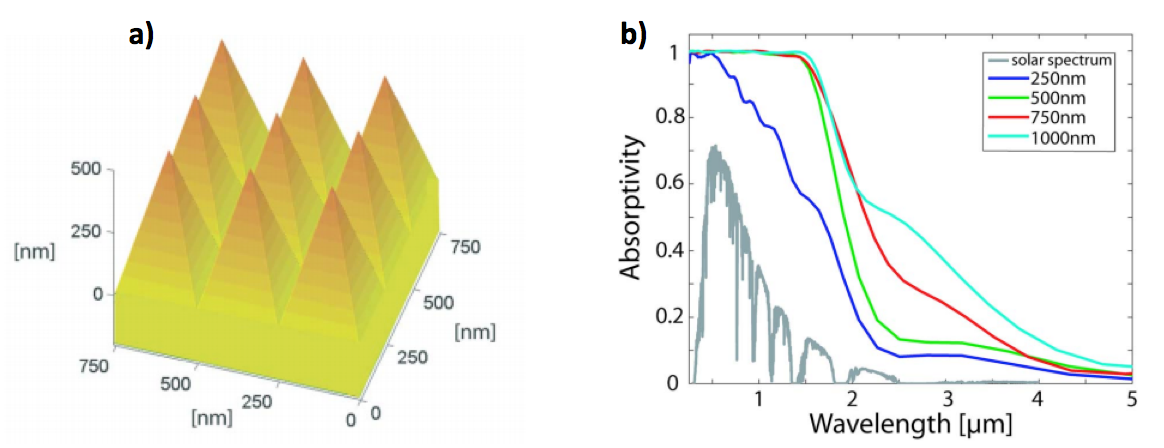
\includegraphics[width=\textwidth]{FDTD_Modeling}
        \caption{\label{FDTD_Structures}  Illustration of a tungsten structure whose
absorptivity can be tuned by patterning of the surface.  In this example, the tungsten
structure is patterned with nanopyramids with various pyramid heights and with period fixed
at  250 nm.  A representative structure with a pyramid height of 500 nm is shown in {\bf (a)}.
Absorptivities of textured tungsten structures
are plotted in {\bf (b)} for a variety of pyramid heights with the period of the pyramids
fixed at 250 nm.  The finite-difference time-domain (FDTD) method
was used to compute the absorptivities shown in {\bf (b)}.  
Figures reproduced from~\cite{RF_OptExp_2009} with permission.}
\end{figure}


\subsection{Design of patterned structures for absorption enhancement using the FDTD method}
Extensions of the previously-discussed multi-layer planar structures involve introducing geometric features in the
lateral dimension(s).  These types of structures include 2D and 3D photonic crystals, metasurfaces, metamaterials, and random-textured materials.
FDTD can be a powerful tool for designing these types of structures, and can be particularly efficient when symmetry and/or periodicity can be
exploited.  Often, these sorts of patterned materials are desired to enhance the absorption of visible light, for example, to design a perfect
absorber across the solar spectrum for solar thermophotovoltaic applications.  For such an application, the transmission, reflection, and
absorption can be computed across the spectrum as features of the surface are varied.  This procedure is illustrated in Figure~\ref{FDTD_Structures} (a) and (b), where the absorptivity of a tungsten surface patterned with pyramidal structures is computed by the FDTD method~\cite{paper1_ref4}. Similarly, Atwater and co-workers
have employed FDTD simulation to design ultra-thin patterned surfaces that behave as broad-band
``super absorbers" capable of enhancing conversion efficiency in
thin-film PV materials~\cite{AFB_NatComm_2011}.  Several of the current authors have utilized FDTD simulations to 
study and
design tungsten absorber surfaces patterned with nanocones 
with absorption efficiencies of 80\%~\cite{me1} (see Table 1),
as well as tungsten blazed grating emitter surfaces with spectral efficiencies of 59\%~\cite{me2} (see Table 2).

Many codes like Lumerical~\cite{lumerical}, a commercial-grade
FDTD simulator, and MEEP~\cite{Meep}, an open-source FDTD code, have scripting
capabilities and other built-in tools to perform sweeps and optimizations over system variables, including material constants and geometric
parameters.  
These sorts of scripting interfaces also allow the computation of more sophisticated quantities; for example, the net energy flux between isolated
structures may be desired to optimize near-field radiative heat transfer~\cite{datas2013}.

\subsection{Discrete Dipole Approximation}

Several computational methodologies for solving Maxwell's equations in the frequency domain are also available, and here we focus on the Discrete
Dipole Approximation (DDA), which is particularly useful for problems involving scattering and light absorption from
particles.  The idea behind DDA is to represent scattering structures by an array of $N$ dipoles.  
It is important to note that in practice $N$ is generally large, i.e. the particle or particles
in the problem are being described by many dipoles filling their volumes 
and so that multipolar
interactions can be correctly described.  DDA is thus routinely used as a rigorous 
computational electrodynamics
method and so its name is somewhat deceptive.

In DDA, each dipole has a polarization given by 
${\bf P}_j = \alpha_j {\bf E}_j$, where ${\bf E}_j$ is the electric field 
at the discrete point occupied by dipole $j$, and $\alpha_j$ is the polarizability of dipole $j$, which 
is determined from the permittivity of the material being modeled~\cite{DF_JOptSocA_1994}.  The electric field at the position $j$ of a given dipole is expanded as
\begin{equation}
{\bf E}_j = {\bf E}_{inc,j} - \sum_{k \neq j}^N {\bf A}_{j,k} {\bf P}_k.
\end{equation}
The incident field (${\bf E}_{inc,j}$) has the form of a monochromatic plane wave, and the product
$-{\bf A}_{j,k} \: {\bf P}_k$ gives the electric field at point $j$ due to the polarization at point $k$; hence, the matrix {\bf A} carries information about
the geometry and polarizability of the dipoles.   
The polarization is found by solving the system of linear equations given by
$\sum_{k=1}^N {\bf A}_{j,k} \: {\bf P}_k = {\bf E}_{inc,j}$, where the diagonal elements of ${\bf A}$ have the known form
${\bf A}_{jj} = \alpha_j^{-1}$.
Iterative methods are used to solve this equation,
leading to overall quadratic scaling of
the computational effort with the number of dipoles~\cite{DF_JOptSocA_1994}. 
The optical cross
sections may be written 
in terms of the polarization of the dipoles~\cite{DF_JOptSocA_1994}.

In general, high resolution can be obtained for small structures with a relatively small number of
dipoles, and so DDA can be extremely efficient for modeling the optical properties of nanoparticles.  DDAs formulation in the frequency domain also
makes it more convenient than FDTD for modeling materials whose permittivity depends strongly on frequency since the permittivity as a function of
frequency can be fed directly into the simulation.  While scattering is solved for one frequency at a time, DDA can be run in parallel over the
desired frequency range.  One considerable drawback is that convergence of the DDA method, both in terms of the number of iterations for
solving the linear equations and in terms of the accuracy of the polarization with respect to the number of dipoles, can be quite
challenging for materials with large real or imaginary components of refractive index~\cite{YMH_PRE_2010}.  Silver is a classic material for which DDA modeling presents a particular challenge at visible frequencies.

Interesting recent developments in DDA of relevance to the problems of concern in this review include
variations of DDA that are capable of describing particle-surface interactions \cite{loke2010}
and near-field radiative heat transfer \cite{edalatpour2014}.

\subsection{Design of nanostructures for near-field enhancement of solar energy conversion using the DDA method  }

Concentration of incident optical energy into the near-field of localized surface plasmons supported by nanostructures can also be leveraged to enhance
solar conversion efficiency in PV materials.  This approach is complementary to the one discussed with anisotropic scattering because it
exploits the absorption of the nanostructure(s) rather than the scattering.  The optical energy concentrated in the near-field of the
plasmon can directly excite particle-hole pairs in a PV material with high efficiency if the absorption rate of the PV material is 
larger than the plasmon damping rate (equivalently, the inverse lifetime of the plasmon excitation)~\cite{AP_NatMat_2010}.  Therefore, nanoparticle systems with
high near-field intensities and long plasmon lifetimes are ideal for these applications.  The large cross sections of plasmonic particles
can also be leveraged to increase absorption efficiency in absorber structures in STPV applications.  DDA methods can efficiently compute
near-field distributions, absorption cross sections, etc, for multiple particles with complex geometries and sharp asperities that are separated by small-gaps,
which are structures that typically give rise to exceptional near-field enhancement and large absorption cross sections.  
Plasmon lifetime information can be obtained
from a Fourier transform over the absorption spectrum that is generated directly by DDA simulations run over a desired frequency range.
Because the DDA method captures the fully coupled optical response of assemblies of nanostructures, it could be used to obtain 
an exact description of the absorption efficiency of the distribution of core-shell nanoparticles leveraged by Halas and co-workers
for absorption enhancement~\cite{CH_APL_2006} (see Figure~\ref{Halas}).


\subsection{Summary and outlook for theoretical design methodologies}
We have described a number of powerful theoretical methodologies that can be put to use to understand, predict, and even tailor the optical
response of systems of simple or complex nanostructures.  The use of these methods, along with the ingenuity of many researchers, has
allowed the design of many novel and useful systems for radiative control.  However, as will be discussed in more detail in the remaining sections, 
overall conversion efficiencies of TPV/STPV systems often fall around 3-8\%,  well short of the theoretical limit of 85\%.  A significant challenge remains in integrating
various theoretical methodologies to model and optimize global device performance~\cite{g4,g9}.
In principle, nanostructured systems may be designed or discovered by coupling the various electrodynamics modeling approaches described above 
to global optimization methods.  Generally, an appropriate figure-of-merit to be maximized is identified, e.g. the spectral efficiency which will
be discussed in detail later, and repeated calculations of the figure-of-merit are carried out while adjusting the features of the nanostructure until 
a global optimum is found.  A plethora of multi-parameter optimization methods are available and have been used in the context of optimizing the 
optical response of nanostructures, including clustering algorithms~\cite{g4}, the Simplex method~\cite{Simplex, CH_APL_2006}, genetic algorithms~\cite{ga,DB_JApplPhys_2007}, 
particle swarms~\cite{NDJ_JApplPhys_2012, ParticleSwarm}, and Gaussian
process modeling~\cite{miller1}.  Certainly one
challenge is that an integrated TPV/STPV system must couple together various optical modalities for absorption and emission.  Usually, this requires
abandoning exact analytical approaches in favor of approximate (e.g. perturbative) analytical approaches like coupled-mode theory.  Alternatively,
researchers must rely on the use of the numerical methodologies described above, 
though this may
prove daunting from a computational point of view due to the multi-scale nature of these systems.
Global system optimization must also include considerations like thermal management along with electrodynamics, as the
requisite operating temperatures can lead to oxidation or deformation of the
constituent structures and degradation of the device performance.  
Consideration of these various system parameters creates a highly heterogeneous optimization problem
and presents significant challenges for global optimization.  
However, several authors including Celanovic and co-workers~\cite{g4}
as well as Wang and co-workers~\cite{g9} have taken on the challenge of designing systems with optimal device consideration, which have led to device efficiencies approaching 3\% and 
10\%, respectively. Considering recent interest in exploiting near-field radiative heat-transfer to enhance
TPV/STPV power and conversion efficiency~\cite{NearFieldConcentrated,SZF_NatNano_2016, KJ_SciRep_2016}, we anticipate that modeling methods that utilize
fluctuational electrodynamics~\cite{rodriguez2011,datas2013,didari2014,didari2015,edalatpour2014} will become increasingly important.
Similarly, appropriate modeling of radiative, electrical, and thermal loss mechanisms will be critical for helping to bridge
the gap between theory and experiment in the field~\cite{BDB_SciRep_2015}.
  
\section{Large area fabrication of optical nanostructures}
\subsection{Direct laser writing and laser interference lithography}
A high power laser beam focused to sub-micron dimensions allows direct 
ablation of surface material,  as shown in Figure \ref{gfig12_comb}(a), to form periodic or non-periodic structures.   Alternatively, selective exposure of a 
photoresist can create feature sizes of about 0.5 microns~\cite{g29}. 

\begin{figure}[ht!]
	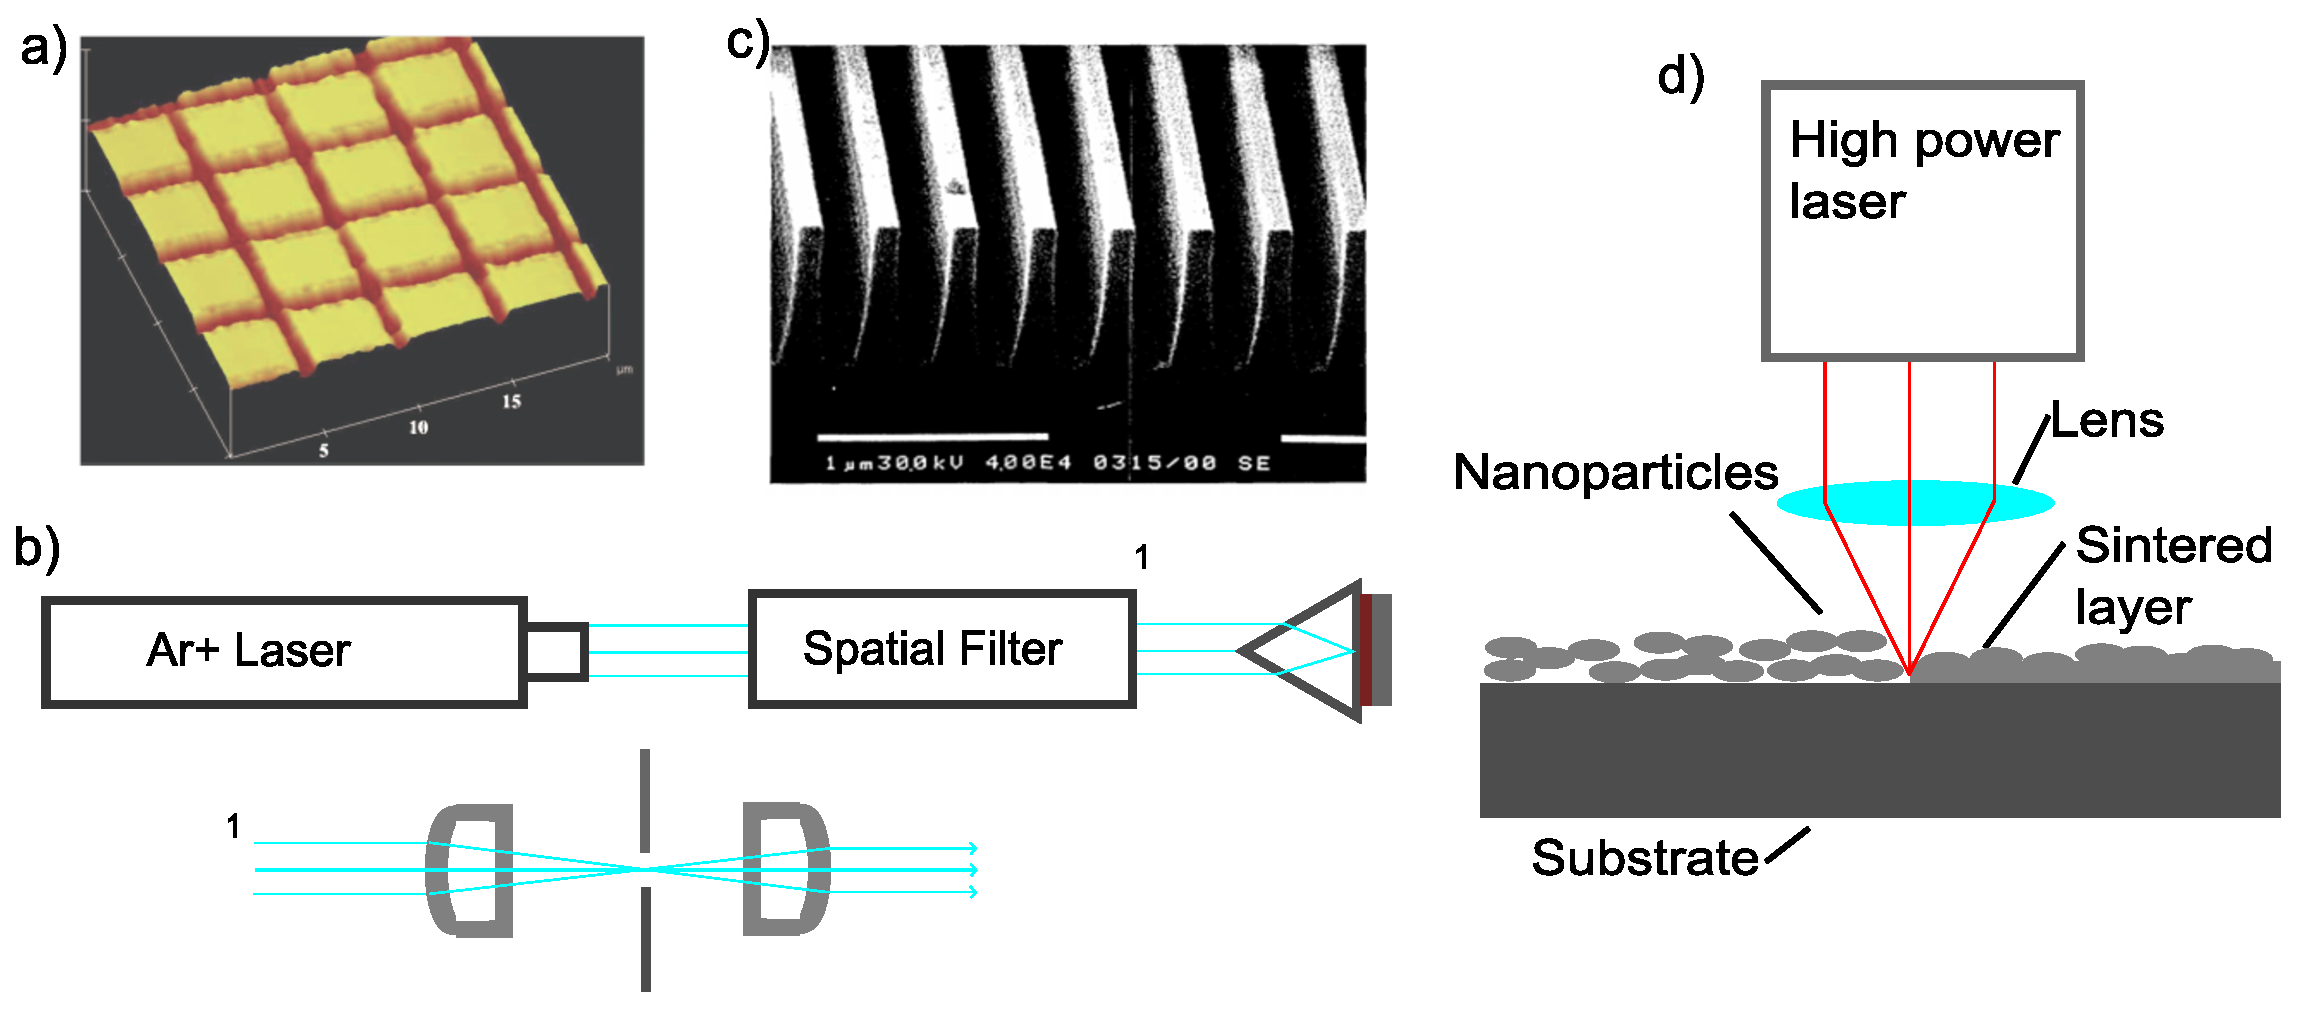
\includegraphics[width=\textwidth]{gfig12_comb}
	\caption{\label{gfig12_comb} a) AFM photograph of a micromachined double periodic structure with line-widths less than a micron \cite{g29} (reproduced with permission), b) Experimental setup for laser interference lithography, c) SEM image of gratings fabricated by laser interference lithography and etched into quartz \cite{g30} (reproduced with permission), and d) experimental setup for laser sintering of nanoparticles.} %
\end{figure}

To obtain feature sizes of few hundred nanometers over a large area, laser interference lithography is ideal ~\cite{g30}. In interference lithography, a laser beam is split into two components, which can be recombined to form an interference pattern,  as shown in Figure \ref{gfig12_comb}(b). 

The period, $P$,  of the grating is determined by $P =\frac{\lambda}{2n\sin(\theta)}$ where  $\lambda$ is the wavelength of the laser light, $n$ is the refractive index of the medium and $\theta$ is the angle between two beams. For a wavelength of 442 nm, a surrounding medium index of 1.5, and an angle between the two beams of 60 degrees, line-widths of about 200 nm will be generated.  
Figure \ref{gfig12_comb}(c) shows a scanning electron microscope (SEM) image of the periodic pattern obtained with a He-Cd laser. This technique can allow the fabrication of large area patterns on various substrates. An exposed photoresist mask is used to etch the pattern on the substrate materials. 

This method will be well suited for the fabrication of spectrally-selective surfaces as 
needed for STPV and TPV systems.  The selective spectral emission wavelength and the 
efficiency of the emission can be controlled by the period, height and spacing between lines.

\subsection{Laser sintering of nanoparticles}
To achieve nanoscale roughness, nanoparticles dispersed in a liquid can be coated on a substrate~\cite{LaserProcessing}. A laser sintering process is then used to fuse the nanoparticles together by the high temperature generated by laser light absorption. In this process, the nanoparticles also get bonded to the substrate. The laser sintering process is shown in Figure \ref{gfig12_comb}(d).  By controlling laser processing parameters such as optical power, scan speed, and beam overlap, different surface morphologies can be achieved. This fabrication method is well suited for solar thermal applications where high solar absorptance and low thermal emission is required.

\subsection{Glancing angle deposition (GLAD)}
Highly light-absorbing surfaces can be generated by micro-scale roughness 
due to the multiple reflections within such surfaces that effectively trap the incident light.  
Thin films of various materials, when deposited at large angles of incidence
relative to the substrate and under vacuum conditions, give rise to cone like 
structures as shown in Figure \ref{gfig45_comb}(a)~\cite{GlancingAngle}. The deposited films look black to the 
naked eye because of their extremely high optical absorption.  The absorption efficiency of 
these structures can be controlled by the height of, and spacing between, the pillars.  
The glancing angle deposition method can be used to enhance solar light absorption 
and to fabricate spectrally-selective surfaces

\begin{figure}[ht!]
	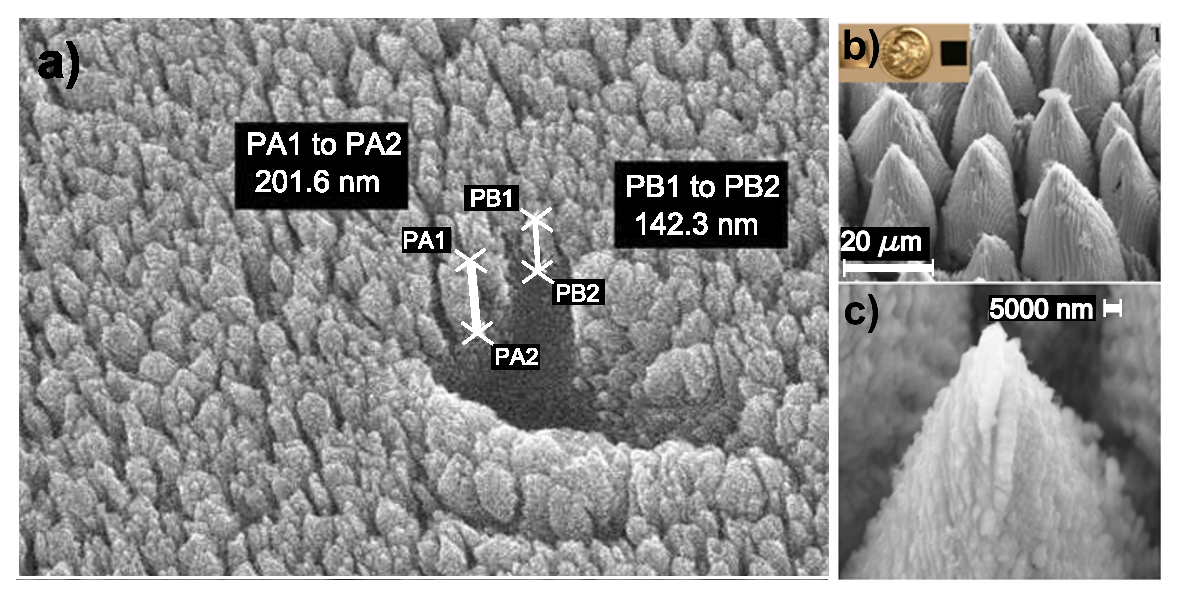
\includegraphics[width=0.65\textwidth]{gfig45_comb}
	\caption{\label{gfig45_comb} a) SEM image of GLAD structures (reprinted with permission) \cite{gfig4ref} and b) and c) SEM images of a laser micro/nano textured Ti surface (reprinted with permission) \cite{g28}.} %
\end{figure} 

\subsection{Laser micro/nano textures}
Micro- and nano-textured surfaces can be obtained when a high power laser beam is 
focused on a substrate and laser processing is carried out within a certain power 
and scan speed range \cite{g28}.  The details of the texture, including height and spacing, can be controlled by laser processing parameters.  The properties of the textured surface allow control over the absorption efficiency of the surface. Figure \ref{gfig45_comb}(b) and \ref{gfig45_comb}(c) show SEM images of a laser microtextured Ti surface. 

Multi-layer thin films composed of metal dielectric layers can also be designed such that high optical absorption can be achieved.  Reciprocally, the emissivity of multi-layer structures can be tuned over a narrow spectral range. Figure \ref{gfig_surfs}(c) shows an example of thin film structure to control the emission properties. 

The high solar radiation absorption can be achieved by fabrication techniques such as metal-dielectric multi-layer structures, surface microtexturing and by the use semiconductor-metal layer structures. The spectral selective emittance can be achieved by fabrication of photonic crystal structures using standard optical or e-beam lithography method or by the use of periodic/non-periodic submicron surface textures.  The microtexture fabrication method is suited to achieve black surfaces with extremely high (\textgreater95\%) light absorption over broad wavelength and incident angle ranges.

\section{Solar energy conversion applications}
\subsection{Solar thermal}
Solar thermal (ST) systems are solar powered devices that generate energy via a heat engine.  Incoming solar energy is concentrated on an absorbing surface, which is heated to high temperatures.  A heat exchange fluid is then used to draw energy from the absorbing surface to the heat engine.  Since heat engines can be more efficient at higher operating temperatures, ST systems operate at high temperatures, up to 1000$^\circ$C.

Operating at such high temperatures means that there will be a large amount of thermal emission from the absorbing surface, resulting in a loss of energy.  To reduce this loss, the thermal emittance of the absorbing surface must be minimized.  Here, we will define $\epsilon_{abs}$ as the thermal emittance of an absorbing surface held at a specific temperature relative to the thermal emittance of a blackbody held at the same temperature.  This means that an absorbing surface with an $\epsilon_{abs}$ of 0.5 at 1000$^\circ$C would have half the thermal emission of a blackbody at 1000$^\circ$C.  Note that the $\epsilon_{abs}$ of a surface can change drastically with temperature if its reflectivity and absorbance change for different wavelengths of light.  This is because the spectral composition of blackbody radiation changes with temperature.  At the same time, the solar absorptance ($\alpha_{sol}$) of the surface must be maximized to ensure a high power input into the device.

For a surface to have high $\alpha_{sol}$ and low $\epsilon_{abs}$, it must have a low reflectance and high absorbance in visible wavelengths (where most solar light is located), and a high reflectance in the near infra-red (NIR) region (where most thermal emission is located).  This is a type of spectrally selective surface.  These surfaces must also remain stable under the high operating temperatures found in ST systems.  The relative importance of high $\alpha_{sol}$ and low $\epsilon_{abs}$ can change due to changes in system parameters.  For example, higher operating temperatures increase thermal emission and place more importance on achieving a low $\epsilon_{abs}$, while higher solar concentrations result in achieving a high $\alpha_{sol}$ being more important.

Spectrally-selective surfaces are much studied in ST research 
because they can lead to high-efficiency systems.  While coatings for lower (\textless500$^\circ$C) temperatures have been extensively studied, they are generally not suitable for high temperature operation due to a lack of thermal stability \cite{A1}.  Some research has attempted to use silicon or germanium based absorbers, but their high solar reflectance necessitates the use of broad-band anti-reflective coatings which results in high $\epsilon_{abs}$, and their performance degrades at high temperatures due to oxidation \cite{A2}. 

Stacks of layered dielectric and metallic films can be used to control the reflectance of structures via multiple reflections and interference effects \cite{A3}.  Many different materials have been investigated for this purpose, including stacks using tungsten, molybdenum, titanium oxide, and magnesium fluoride that had an $\epsilon_{abs}$\textless7\% and $\alpha_{sol}$\textgreater94\% \cite{paper1_ref7,stacks2, A2}.  Unfortunately, fabrication of these surfaces requires vacuum deposition of multiple layers with precise thickness, which can be difficult.

Ceramic-metal composites (cermets) consist of metallic particles in a dielectric host that are often used as spectrally selective surfaces in ST applications.  The metallic particles in the cermet layer result in high $\alpha_{sol}$ due to multiple reflections, and they are typically used on metallic substrates with high IR reflectance, resulting in low $\epsilon_{abs}$ \cite{A2,A4,A5,A6,A7,A8,A9,A10}.  The disadvantages of cermets include sensitivity to oxygen at high temperatures and the requirement for vacuum fabrication methods.

Nanotextured surfaces can be stable at high temperatures when they are 
formed from high melting point metals such as tungsten and tantalum and are coated with a protective oxide \cite{paper1_ref5}.  They also lend themselves to fabrication using the methods described in this report.  Because these methods take advantage of surface geometry, they do not require multiple materials, resulting in a high thermal stability.  Indeed, nanostructures of tungsten coated with a protective hafnium coating have been shown to be stable to temperatures of 1100 $^\circ$C in air \cite{paper1_ref5,Therm_stabil_W_microstructures}.  Tantalum photonic crystals have also been reported to be stable at temperatures of over 1000$^\circ$C \cite{photonic_crystal_rev}.

Periodic sub-wavelength gratings on tungsten substrates have been fabricated with an $\alpha_{sol}$ of 82\% and $\epsilon_{abs}$ of 5.6\% at 770$^\circ$C and were experimentally verified to be 
stable up to temperatures of 900 $^\circ$C \cite{A13}.  These structures cause standing wave resonances that can be tuned for solar absorption.

Sub-wavelength roughness on metallic substrates can also increase solar absorbance due to the surface acting as a graded index medium \cite{A13,A19}.  The $\epsilon_{abs}$ of these surfaces can be kept low because NIR wavelengths are much longer than the dimensions of the roughness, so the surface appears smooth \cite{A14}.  An advantage of these types of structures is that they do not require periodicity, and randomness can in fact be an advantage \cite{me1}.  Simulations have shown pseudo-random nanocones on a tungsten substrate to have an $\alpha_{sol}$ of 97\% and $\epsilon_{abs}$ of 16\% at 1400 $^\circ$C \cite{me1}.  Experimental data on surface roughness created by laser-sintering of nanoparticles have shown an $\alpha_{sol}$ of 83\% and $\epsilon_{abs}$ of 11.6\% \cite{g21}.

\subsection{Solar thermophotovoltaics}
Typical STPV systems consist of an absorbing/emitting structure that is held under vacuum to reduce convective losses and increase thermal stability~\cite{global_opt, convection}.  Then, sunlight is focused on the absorbing surface of the structure, where it is absorbed and converted into thermal energy.  This results in the absorbing/emitting structure becoming very hot, with temperatures up to 1750 K common in these systems.  As the system temperature rises, it begins to emit a large amount of thermal radiation.  The portion of thermal energy that is emitted by the emitting surface can then be collected by a PV cell and converted into electrical energy.  An additional advantage of STPV systems is their ability to store absorbed energy as heat, which is more efficient than battery storage with traditional PV cells.  STPV technology can also be easily adapted to thermophotovoltaic (TPV) systems, which operate similarly but use a burning fuel or waste heat as a thermal source instead of the sun. By transforming the incoming solar radiation from a broad-band source to a more narrow-band one, STPV systems can operate at efficiencies exceeding the Shockley-Queisser limit of 44\% for silicon PV cells operating under diffuse radiation~\cite{SQ}.  In fact, the upper {\it theoretical} limit for STPV system efficiency is 85.4\%~\cite{A2}.

\begin{table}
	\caption{Efficiency, relative solar absorption, and relative thermal emission at a temperature of 1700 K of selected absorbing surfaces.}
	\label{abs_eff_table}
	\begin{center}
		\begin{tabular}{|llll|}
			%\begin{tabular}{|p{5.3cm}|p{2.6cm}|}
			\hline
			Absorber type & Absorber efficiency & $\alpha_{sol}$ & $\epsilon_{abs}$\\
			\hline	
			Ideal solar absorber & 0.83 & 0.87 & 0.04\\
			Pseudo random nano-cones in W & 0.80 & 0.97 & 0.16~\cite{me1}\\
			W pyramidal nanostructures & 0.79 & 0.92 & 0.13~\cite{paper1_ref4}\\
			Mo-SiO$_2$ cermet & 0.77 & 0.93 & 0.16~\cite{cermet6}\\
			Carbon nanotubes & 0.74 & 0.99 & 0.95~\cite{MIT_paper,nnnNature}\\
			1-D photonic crystal on W & 0.74 & 0.80 & 0.06~\cite{SKY_JPE_2015}\\
			Blackbody absorber & 0.73 & 1.00 & 1.00\\
			Anti-reflection coating on W & 0.67 & 0.73 & 0.05~\cite{SKY_JPE_2015}\\
			W cavities & 0.59 & 0.74 & 0.15~\cite{exp_russia}\\
			Surface-relief grating on W & 0.49 & 0.53 & 0.05~\cite{paper1_ref6}\\
			Bare W & 0.41 & 0.44 & 0.04~\cite{palik}\\
			\hline
		\end{tabular}
	\end{center}
\end{table}

The absorbing surfaces for STPV devices are similar to those used in ST systems, although higher operating temperatures (up to around 1750 K) 
make thermal stability a more prominent concern, and high levels of solar concentration (\textgreater4000) make a high $\alpha_{sol}$ of 
paramount concern.  This means that nanotextured absorbing surfaces are a very good match for these systems.  Most experimental STPV systems 
to date have utilized blackbody absorbing surfaces \cite{exp_tokyo,exp_madrid,exp_russia,MIT_paper}, leaving room for much improvement by using 
selective absorbing surfaces. Recent results have reported record efficiencies~\cite{g11,SKY_JPE_2015} using both 
selective absorbers and selective emitters. A yttria-stabilized zirconia and tungsten stack was used as a selective absorber in an experimental system~\cite{SKY_JPE_2015}, 
but while it's thermal emission was low, its performance was hindered by a low $\alpha_{sol}$ of 80\%.  Simulations of various surfaces 
have shown large gains in system efficiency from the use of nanotextured selective, such as pseudo-random 
nanocones with an $\alpha_{sol}$ of 97\% and $\epsilon_{abs}$ of 16\% \cite{me1}, or pyramidal nanostructures in tungsten 
with an $\alpha_{sol}$ of 92\% and $\epsilon_{abs}$ of 13\% \cite{paper1_ref4} but none have been experimentally 
demonstrated in a working STPV system to date \cite{paper1_ref5,paper1_ref6}.

Various methods of evaluating STPV system performance exist, but in this work we will focus on the relative efficiencies of the individual surfaces of an STPV device.  This allows us to directly compare different methods of making selective absorbing and emitting surfaces.  Many parameters in STPV systems can effect the performance of these surfaces, so an operating temperature of 1450$^\circ$C, a solar concentration of 2500, and a GaSb solar cell are assumed here due to their prevalence in STPV systems~\cite{exp_tokyo,exp_madrid,exp_russia,me1,me2,RF_OptExp_2009}.  This provides for a good relative comparison of different surfaces, although it is not a measure of overall device efficiency.

Table \ref{abs_eff_table} shows the $\alpha_{sol}$ and $\epsilon_{abs}$ of some absorbing surfaces, as well as a calculated surface efficiency.  The quantity $\eta_{abs}$ is given by
\begin{align}
\label{overall_sss_eq}\eta_{abs}(T)& = \frac{\int_{0}^{\infty}\left\{E_{inc}(\lambda)\alpha(\lambda)-\epsilon(\lambda)B(\lambda,T)\right\}d\lambda}{\int_{0}^{\infty}E_{inc}(\lambda)d\lambda}\\
\label{e_incident}E_{inc}(\lambda) &= C \: \eta_{conc} \: E_{sun}(\lambda),
\end{align}
where $\alpha(\lambda)$ is the spectral absorption of the surface, $\epsilon(\lambda)$ is the spectral emittance of the surface, $C$ is the concentration ratio of incoming sunlight, 
$\eta_{conc}$ is the solar concentration efficiency, $E_{sun}(\lambda)$ is the 
spectral irradiance of the sun at the earth's surface, $B(\lambda, T)$ is 
Planck's law for blackbody radiation, and $E_{inc}(\lambda)$ is the spectral 
energy incident on the absorbing surface.

For emitting surfaces, a similar approach to absorbing surfaces can be taken, but with a focus on low reflectance in a narrow peak near a specific wavelength (which depends on the bandgap energy of the PV cell used), as opposed to a broad low reflectance band in the visible region.  To accurately compare emitting surfaces, their spectral efficiency is used.

The spectral efficiency is given by~\cite{me2}:
\begin{equation}\label{SpecEff}
SE = \frac{  \int_0^{\lambda_{bg}} \frac{ E_{bg} }{E_{\lambda}} \: B(\lambda, T) \: \epsilon_S (\lambda) \: d\lambda }
{\int_0^{\infty} B(\lambda,T) \: \epsilon_S (\lambda) \: d\lambda}
\end{equation}
where $E_{bg}$ is the bandgap energy of the PV cell, $E_{\lambda}$ is the energy of a photon with wavelength $\lambda$, and $\epsilon_S (\lambda)$ is the spectral emissivity of the emitting surface, approximated as the surface's absorptivity.  This gives the relative efficiency of the emitting surface, but does not represent an overall system efficiency.

Two structures work particularly well for this purpose: dielectric-metal stacks and 2-D or 3-D photonic crystals.  A yttria-stabilized zirconia (YSZ) and tungsten stack was able to achieve highly selective emission and experimentally demonstrated to be stable at temperatures up to 1350 $^\circ$C \cite{SKY_JPE_2015}.

\begin{table}
	\caption{Optical efficiency of selected emitting surfaces at 1700 K~\cite{me_thesis}.}
	\label{FOM_table}
	\begin{center}
		\begin{tabular}{|lc|}
			\hline
			Emitter type & $\eta_{emit}$\\
			\hline	
			Ideal emitting surface & 0.84 \\
			Periodic hole array on W & 0.64 (simulated)\\
			Blazed grating on W & 0.59 ~\cite{me2} \\
			Anti-reflection coating on W & 0.59 (simulated) \\
			Complex square grating on W & 0.53~\cite{paper2_ref14}\\
			1-D photonic crystal on W & 0.53~\cite{SKY_JPE_2015}\\
			Micro-cavity in W & 0.51~\cite{paper2_ref6} \\
			{A}l$_2${O}$_3$/{E}r$_3${A}l$_5${O}$_{12}$ eutectic composite & 0.41~\cite{exp_tokyo}\\
			Blackbody emitter & 0.29\\
			\hline
		\end{tabular}
	\end{center}
\end{table}

Many nanotextured emitting structures have been simulated to be extremely efficient \cite{paper2_ref13}.  These include blazed gratings on tungsten \cite{me2}, complex square gratings on tungsten \cite{paper2_ref14}, micro-cavities in tungsten \cite{paper2_ref6}, tungsten surface gratings \cite{paper1_ref6}, 3-D photonic crystals \cite{paper2_ref10}, and metamaterials \cite{meta}.  Table \ref{FOM_table} shows the spectral efficiencies of some of these surfaces.  This shows a large increase in efficiency for selective emitters over blackbody emitters.  While experimental systems using these structures have not yet been realized, they promise large efficiency gains for the future.  Table \ref{STPV_sys_table} shows the electrical efficiencies of some simulated and experimental STPV systems. 
The simulations outlined here show a large difference in predicted efficiency; however, a significant portion of this variation is caused by simulation parameters.  Since there is no standard for simulated STPV systems, some papers use an ideal model where only losses due to the surfaces are accounted for, while others use a more realistic model that encompasses many losses.  Namely, references \cite{RF_OptExp_2009} and \cite{global_opt} assume ideal PV cells, ideal solar concentrators, and assume an ideal view-factor between the emitting surface and solar cells.  References \cite{paper2_ref6}, \cite{me_thesis}, and \cite{NYL_SEMSC_2014} attempt to model PV cell losses and realistic absorbing and emitting surfaces.  Some of the remaining difference between efficiencies in the modeled systems is also due to differences in assumptions between simulations.

Despite the assumptions in these models, they clearly show that nanostructured surfaces are extremely important to ensure adequate spectral selectivity in these systems.  While reference \cite{RF_OptExp_2009} and \cite{global_opt} used many idealities, they clearly show that STPV systems are capable of having efficiencies above the Shockley-Queisser limit for single junction PV cells.  References \cite{paper2_ref6}, \cite{me_thesis}, and \cite{NYL_SEMSC_2014} predict high potential operating efficiencies using realistic operating conditions.  The primary reason that experimental systems lag behind simulations is because a lack of high quality nanostructures in these systems \cite{SKY_JPE_2015,me3}.  The YSZ and W stack used in \cite{SKY_JPE_2015} proved to be a less efficient solution for both the absorbing and emitting surfaces than other surfaces examined in this article.  In \cite{me3}, secondary, less efficient surfaces had to be used for both the absorbing and emitting structures due to fabrication problems. References \cite{SKY_JPE_2015,MIT_paper,nnnNature} uses a blackbody absorbing surface, which results in suboptimal efficiency.  Still, these devices are able to achieve very high operating efficiencies by operating at low temperatures to mitigate thermal emission from the absorber and by using nanostructured emitting surfaces.  The inclusion of an extra filter on emitted light to reduce losses in the emitting surface can also increase efficiency\cite{nnnNature}.  Still, theoretical efficiencies are much higher than experimental ones. This points to a large increase in efficiency that can be achieved by using nanostructures to close the gap between experimental and theoretical devices.  The simulation and fabrication methods outlined in this paper show that this is possible.

\begin{table}
	\caption{Efficiency of selected STPV systems.}
	\label{STPV_sys_table}
	\begin{center}
		\begin{tabular}{|lllll|}
		\hline
		Absorbing surface & Emitting surface & PV cell & Temp. (K) & Efficiency (\%)\\
		\hline
		\multicolumn{5}{c}{Experimental systems} \\
		\hline
		Carbon nanotubes	& Si/SiO$_2$ stack	& InGaAsSb & 1200 &	6.8 \cite{nnnNature} (2016)\\
		Laser-textured W & W with Si$_3$N$_4$ & GaSb & 1777& 6.2 \cite{me3} (2015)\\
		with Si$_3$N$_4$ coating & coating &&&\\
		Carbon nanotubes & Si/SiO$_2$ stack & InGaAsSb & 1285 & 3.2 \cite{MIT_paper}  (2014)\\
		YSZ and W stack	& YSZ and W stack	& GaSb & 1640 &	2 \cite{SKY_JPE_2015} (2015)\\
		Graphite & W with HfO$_2$ & Ge & $\sim$1700 & 0.8 \cite{exp_madrid}  (2012)\\
		& coating &&&\\
		Tungsten cavity & Thin W film & GaSb & $\sim$2000 & 1 \cite{exp_russia} (2007)\\
		Graphite & {A}l$_2${O}$_3$/{E}r$_3${A}l$_5${O}$_{12}$ & GaSb & Unmeasured & 0.02 \cite{exp_tokyo} (2000)\\
		& composite &&&\\
		\hline
		\multicolumn{5}{c}{Simulated systems} \\
		\hline
		Pyramidal W & Si/SiO$_2$ stack & GaSb & 6000 & 49~\cite{RF_OptExp_2009}\\
		nanostructures &&&&\\
		Blackbody absorber	& Monochromatic & Ideal cell	& 2872 & 45.3~\cite{global_opt}\\
		& emitter &&&\\
		Selective absorber	& W surface grating & GaSb & 1920 & 23.4~\cite{paper2_ref6} \\
		& with Si/SiO$_2$ filter & & &\\
		Periodic hole &	Pseudo-random & GaSb	& 1700 &	14.4~\cite{me_thesis}\\	
		array on W	& cones on W&&&\\	
		2D Ta photonic & 2D Ta photonic & InGaAsSb & 1400 & 10~\cite{NYL_SEMSC_2014}\\
		crystal& crystal &&&\\
		\hline
		\end{tabular}
	\end{center}
\end{table}

Thermophotovoltaic (TPV) systems are another important area for harvesting waste heat energy. The reported efficiency of TPV systems is low at around few percent. However, as demonstrated by Bermel et al. \cite{g4} by using spectral selective surfaces the calculated efficiency can be  very high (26.2\%). The calculation was based on operating temperature of 1200$^\circ$C. Similarly, Foley et al.~\cite{FUS_OptExp_2015} has shown in the paper as part of this special issue that by using metal (Ag)-dielectric (Si$_3$N$_4$) structure the calculated  efficiency of 10\% can be achieved at low operating temperature of 1000$^{\circ}$C.  It can also be further enhanced by using selective filters and operating at 1200$^\circ$C. 

\section{Conclusions}
We discussed a variety of modeling and fabrication techniques for controlling light 
absorption and emission by nanostructures.   Such control is important for solar and 
thermal energy conversion devices including traditional photovoltaic (PV), 
solar thermal (ST), and solar thermophotovoltaic (STPV) devices. 
The use of thermal energy conversion in particular, 
can circumvent some efficiency limitations on standard PV cells.  We 
anticipate that significant efficiency improvements can be achieved in this area 
by building on the techniques discussed here.  For example, while ST systems 
are already achieving high efficiencies in commercial use, experimental 
TPV and STPV efficiencies remain low.  The primary cause of lowered device 
efficiency is lack of control over the spectral emissivity of the 
absorbing and emitting surfaces.  The nanostructures, simulation, and 
fabrication methods highlighted here can be used to greatly increase 
efficiencies in all three of these systems.  
Indeed, simulations of nanostructured devices show that extremely high efficiencies 
exceeding the Shockley-Queisser limit are achievable in TPV/STPV systems.
For example, one of the most promising simulated devices have shown conversion efficiencies of 26.2\% at 
system temperatures of 1200$^\circ$C and a maximum conversion efficiency of 49\% was predicted for system 
temperatures of about 2130 K~\cite{RF_OptExp_2009}.  However, the highest conversion efficiency measured
for an STPV device is about 8\% for 1D photonic crystal structures of composed of tungsten and YSZ at 
device temperatures of 1640 K~\cite{SKY_JPE_2015}.  This large gap in system efficiency is due to the lack of temperature-stable 
nanostructures and high losses in experimental STPV systems.  Future theoretical design methodologies should involve
explicit considerations of aspects like thermal properties of materials and the thermal deformation of 
nanostructures to guide the fabrication of structures that are more robust to thermal degradation.    
Additionally, management strategies including the use of ST systems in tandem with STPV systems to capture waste heat from the STPV device
should be explored.

\section*{Acknowledgments}
We would like to thank the NASA Langley Professor and NSF IUCRC programs for their support of this project.  Part of this work was performed at the Center for Nanoscale Materials, a U.S. Department of Energy, Office of Science, Office of Basic Energy Sciences User Facility under Contract No. DE-AC02-06CH11357.

\bibliography{solar_energy_rev1}

\end{document}
